\chapter{Experiments and Results}
\label{chap:experiments}

This chapter evaluates cascaded image-domain encoder--decoder architectures on a corruption distribution that combines low-dose Poisson noise with the three sinogram-domain physical artifacts introduced in \Cref{sec:meth_compound}. To our knowledge, this joint setting has received limited attention in the literature: low-dose CT benchmarks typically isolate noise, whereas artifact-correction studies usually assume nominal photon flux. The protocol of \Cref{sec:meth_overview} is designed to bridge that gap and provides the experimental setting in which the second contribution of this work---the comparison of independent-stage, end-to-end, and residual cascade formulations---is assessed against matched single-network baselines.

The central finding of the chapter is that a single well-designed encoder--decoder already operates close to the practical image-domain ceiling on this protocol. Adding a second image-domain stage yields only limited benefit unless it is given access to new information. Among the cascade variants, the residual formulation produces a small but consistent improvement, while the gradient analysis later in the chapter helps explain why the end-to-end formulation does not.

\Cref{sec:exp_setup} defines the data, baselines, and evaluation metrics.
\Cref{sec:exp_baselines_table} reports the baseline reference results.
\Cref{sec:exp_cascade} presents the matched-capacity cascade comparison.
\Cref{sec:exp_asymmetric} examines the asymmetric-capacity setting.
\Cref{sec:exp_qualitative} shows representative qualitative examples.
\Cref{sec:exp_gradient} Analyzes per-stage gradient flow.
\Cref{sec:exp_discussion} discusses the implications and limitations of the findings.
%%─────────────────────────────────────────────────────────
%% Experimental setup
%%─────────────────────────────────────────────────────────
\section{Experimental Setup}
\label{sec:exp_setup}

\subsection{Dataset and corruption protocol}
\label{subsec:exp_dataset}

All models are trained and evaluated on the LoDoPaB-CT benchmark~\cite{Leuschner2021}, using the official train\,/\,validation\,/\,test split (\num{35820}\,/\,\num{3522}\,/\,\num{3553} slices). The corruption protocol described in \Cref{sec:meth_compound} is applied independently to each sample during batch construction. Low-dose Poisson noise is inherited from the LoDoPaB simulator (\(N_0=\num{4096}\) photons per pixel), while the three physical artifacts---motion, ring, and metal---are independently activated by per-sample Bernoulli draws with probabilities \((p_\mathrm{mot}, p_\mathrm{ring}, p_\mathrm{met}) = (0.5, 0.5, 0.3)\).

For the validation and test splits, the per-sample random number generator is seeded as \(\mathrm{seed}+\mathrm{idx}\), so that every method in this chapter is evaluated on an identical set of artifact realizations. All images are displayed using the LoDoPaB intensity window \([0, 0.45]\) on the \(\mu_{\max}\)-normalized scale~\cite{Leuschner2021}.
%%─────────────────────────────────────────────────────────
%% Baselines
%%─────────────────────────────────────────────────────────
\subsection{Baselines}
\label{subsec:exp_baselines}

Three classes of baseline are included in the comparison. The corrupted FBP reconstruction $\mathbf{y} = \mathcal{R}^{-1}\tilde{\mathbf{s}}$ provides the unrecovered input and therefore sets the minimum performance level that any restoration method must improve upon. \gls{bm3d}~\cite{Dabov2007} is applied directly to $\mathbf{y}$ as a classical non-learned reference; its noise parameter is selected by a five-point grid search on the validation set over $\sigma \in \{0.05, 0.075, 0.1, 0.15, 0.2\}$, yielding a best value of $\sigma = 0.10$.

\gls{redcnn}~\cite{Chen2017} is included as a learned single-network reference with \num{1842049} trainable parameters and is trained on the same corrupted/clean pairs as the cascade variants. Finally, a single-stage U-Net identical in architecture to the first stage of each cascade model is trained at two capacities: \emph{U-Net (small)} with \num{1798113} parameters (channel widths $[32, 64, 128, 256]$) and \emph{U-Net (large)} with \num{7184321} parameters (channel widths $[64, 128, 256, 512]$). These two U-Net configurations serve as matched-capacity references for the small and large cascade variants, respectively.
%%─────────────────────────────────────────────────────────
%% Cascade variants
%%─────────────────────────────────────────────────────────
\subsection{Cascade variants}
\label{subsec:exp_variants}

The three coupling formulations introduced in \Cref{sec:meth_arch} are evaluated.

\begin{description}
    \item[Independent-stage (naive).] Both stages are trained simultaneously under the cascade objective, but a stop-gradient operator is applied to $\hat{\mathbf{x}}_1$ at the stage boundary. As a result, Stage~1 is updated only by $\mathcal{L}^{(1)}$, while Stage~2 is updated only by $\mathcal{L}^{(2)}$.

    \item[End-to-end.] Both stages are trained jointly under the weighted loss $0.5\,\mathcal{L}^{(1)} + 0.5\,\mathcal{L}^{(2)}$, and gradients are allowed to propagate through the full cascade.

    \item[Residual.] Stage~2 predicts an additive correction $\hat{\mathbf{r}}_2$ to the Stage~1 output, as defined in \Cref{eq:meth_residual}, and is supervised using the residual loss $\mathcal{L}^{(2)}_{\mathrm{res}}$ from \Cref{eq:meth_loss_residual}. Unless stated otherwise, the reported residual models use the independent-stage training protocol.
\end{description}

Two additional configurations are included to test whether cascade performance is limited primarily by parameter allocation or by the information available to the second stage.

\begin{description}
    \item[Asymmetric capacity.] A small Stage~1 followed by a large Stage~2, and the converse arrangement, are evaluated as defined in \Cref{subsec:meth_asymmetric}. This tests whether redistributing model capacity across the two stages changes the marginal value of the cascade.

    \item[Dual-filter input to Stage~2.] The alternative-filter scheme of \Cref{eq:meth_alt_input} is used, in which Stage~2 receives $\hat{\mathbf{x}}_1$ concatenated with Hann- and Shepp--Logan-filtered FBP reconstructions of the same corrupted sinogram. This provides Stage~2 with additional image-domain information not present in the Ram--Lak input to Stage~1.
\end{description}
%%─────────────────────────────────────────────────────────
%% Evaluation metrics
%%─────────────────────────────────────────────────────────
\subsection{Evaluation metrics}
\label{subsec:exp_metrics}

Evaluation is reported in terms of \gls{psnr}, \gls{ssim}, and root-mean-square error (RMSE),
\begin{equation}
    \mathrm{RMSE}(\hat{\mathbf{x}}, \mathbf{x})
    = \sqrt{\tfrac{1}{HW}\sum_j (\hat{x}_j - x_j)^2}.
    \label{eq:exp_rmse}
\end{equation}
All metrics are computed per slice on the $\mu_{\max}$-normalized image and then averaged over the \num{3553} test slices. Before metric computation, model outputs are clamped to $[0,1]$. For PSNR, the dynamic range is set to $\mathrm{MAX}=1.0$, corresponding to the full $\mu_{\max}$-normalized intensity range of the images. The display window $[0,\,0.45]$ used for visualization~\cite{Leuschner2021, Kiss2024} is a windowing convention only and is not used as the PSNR denominator.

All cascade variants are trained for up to $150$ epochs with early stopping (patience $15$) and AdamW at a learning rate of $3\times 10^{-4}$ using identical seeded corruption draws. Joint losses use equal per-stage weights, $w_1 = w_2 = 0.5$. For the independent-stage variants, the stop-gradient operator at $\hat{\mathbf{x}}_1$ ensures that $\mathcal{L}^{(1)}$ and $\mathcal{L}^{(2)}$ update only the parameters of their respective stages throughout training.
%%─────────────────────────────────────────────────────────
%% Baseline References
%%─────────────────────────────────────────────────────────
\section{Baseline References}
\label{sec:exp_baselines_table}

\Cref{tab:exp_baselines} reports the five baseline reference methods.
Three observations motivate the cascade study that follows. First, the corrupted FBP input is substantially worse than the standard LoDoPaB noise-only setting reported in \cite{Leuschner2021}, confirming that the added physical artifacts materially increase the reconstruction difficulty beyond low-dose Poisson noise alone. Second, BM3D yields only a modest PSNR improvement over the corrupted input, although the gain in SSIM is more pronounced. This is consistent with its role as a classical denoiser that suppresses part of the stochastic noise but leaves structured artifacts largely unresolved.

\begin{table}[!htb]
    \centering
    \caption[Baseline references on LoDoPaB-CT under compound corruption.]{%
        Restoration quality on the LoDoPaB-CT test split
        (\num{3553} slices) under the full compound-corruption
        distribution. PSNR is computed on the $\mu_{\max}$-normalized image with
        $\mathrm{MAX}=1.0$ (full normalized range); model outputs are clamped to $[0,1]$
        before evaluation. The display window $[0,\,0.45]$~\cite{Leuschner2021} is used
        for visualization only and does not affect metric computation.}
    \label{tab:exp_baselines}
    \setlength{\tabcolsep}{6pt}
    \small
    \begin{tabular}{@{}l r r r r@{}}
        \toprule
        Method                              & Params    & PSNR (dB) & SSIM     & RMSE    \\
        \midrule
        Corrupted FBP (input)               & ---       & $21.49$   & $0.4488$ & $0.0869$ \\
        BM3D on FBP~\cite{Dabov2007}        & ---       & $22.14$   & $0.6814$ & $0.0806$ \\
        RED-CNN~\cite{Chen2017}             & $1.84$\,M & $27.03$   & $0.7107$ & $0.0500$ \\
        U-Net (small)                       & $1.80$\,M & $35.39$   & $0.8680$ & $0.0193$ \\
        U-Net (large)                       & $7.18$\,M & $\mathbf{36.11}$ & $\mathbf{0.8772}$ & $\mathbf{0.0178}$ \\
        \bottomrule
    \end{tabular}
\end{table}

Third, RED-CNN improves clearly over BM3D but remains well below the U-Net references, trailing even the smaller U-Net by more than \SI{8}{\decibel} in PSNR. Two architectural factors explain the gap. RED-CNN was originally designed for single-type Poisson noise at a fixed dose~\cite{Chen2017}: its encoder--decoder comprises only five convolutional layers per path without multi-resolution pooling, which limits the receptive field available for suppressing the spatially extended streaks and rings introduced by the compound-corruption protocol. The U-Net's skip connections and three-level pooling hierarchy provide a substantially larger effective receptive field, enabling it to integrate spatial context over the full extent of metal streaks and motion-induced ghosts. Inspection of loss curves (not shown) confirms that RED-CNN converged within the first 30 epochs under the present training protocol, ruling out insufficient training as an explanation for the gap. The two U-Net baselines therefore form the most relevant single-stage references for the cascade comparisons reported below.

\paragraph{Per-slice metric variability.}
All mean metrics reported in this chapter are computed over all \num{3553} test slices, which span a wide range of corruption severities. Per-slice standard deviations, evaluated for the two strongest models (U-Net large and the residual dual-filter cascade), are $\sigma_{\mathrm{PSNR}} \approx \SI{4.4}{\decibel}$ and $\sigma_{\mathrm{SSIM}} \approx 0.12$. These large spreads reflect the inherent variability of the compound corruption protocol: noise-only slices reach up to $\SI{39.6}{\decibel}$ on average, while triple-artifact slices fall to approximately $\SI{33.9}{\decibel}$ (see \Cref{tab:exp_per_artifact}). The mean differences between cascade variants (typically $0.15$--$0.72$\,dB) are therefore small relative to the within-test-set spread. They are, however, consistent across the full \num{3553}-slice evaluation and align with the qualitative and gradient evidence presented in the following sections.
%%─────────────────────────────────────────────────────────
%% Cascade Comparison at Matched Capacity
%%─────────────────────────────────────────────────────────
\section{Cascade Comparison at Matched Capacity}
\label{sec:exp_cascade}
\label{sec:exp_quantitative}

\Cref{tab:exp_cascade} compares the three cascade formulations against the small single-stage U-Net at matched per-stage capacity. All cascade rows use a small$+$small configuration, so any gain over the small single-stage reference reflects the effect of staging rather than a larger first-stage backbone. The large single-stage U-Net is included as an upper reference. For clarity, the table reports only the final cascade output (Stage~2); Stage~1 results are shown separately in \Cref{fig:exp_stage_improvement}.

The ordering in $\Delta$PSNR is unambiguous. Adding a second image-domain stage under the naive independent protocol improves the small U-Net by only $+0.15$\,dB, indicating that a simple serial decomposition yields little benefit on its own. End-to-end coupling increases this gain to $+0.46$\,dB, and the residual formulation increases it further to $+0.54$\,dB. The best matched-capacity result is obtained by the residual cascade with dual-filter input, which reaches $+0.72$\,dB over the small single-stage U-Net and matches the PSNR of the large single-stage reference.

\begin{table}[!htb]
    \centering
    \caption[Cascade comparison at matched per-stage capacity.]{%
        Cascade output (Stage~2) on the LoDoPaB-CT test split. All cascade
        rows use small$+$small per-stage capacity and are compared against
        the small single-stage U-Net. The large single-stage U-Net is
        included as an upper reference. The best result among the
        matched-capacity rows is shown in \textbf{bold}. $\Delta$PSNR denotes
        the gain over the small single-stage U-Net.}
    \label{tab:exp_cascade}
    \setlength{\tabcolsep}{6pt}
    \small
    \begin{tabular}{@{}l r r r r r@{}}
        \toprule
        Method                                     & Params      & PSNR (dB) & SSIM     & RMSE    & $\Delta$PSNR \\
        \midrule
        U-Net (small), single-stage                & $1.80$\,M   & $35.39$   & $0.8680$ & $0.0193$ & --- \\
        \quad Independent (naive)                  & $3.60$\,M   & $35.54$   & $0.8692$ & $0.0191$ & $+0.15$ \\
        \quad End-to-end (naive)                   & $3.60$\,M   & $35.85$   & $0.8730$ & $0.0183$ & $+0.46$ \\
        \quad Independent (residual)               & $3.68$\,M   & $35.93$   & $0.8739$ & $0.0181$ & $+0.54$ \\
        \quad Independent (residual, dual-filter)  & $3.68$\,M   & $\mathbf{36.11}$ & $\mathbf{0.8738}$ & $\mathbf{0.0180}$ & $\mathbf{+0.72}$ \\
        \midrule
        U-Net (large), single-stage (reference)    & $7.18$\,M   & $36.11$   & $0.8772$ & $0.0178$ & --- \\
        \bottomrule
    \end{tabular}
\end{table}

The ordering in $\Delta$PSNR is unambiguous. Adding a second image-domain stage under the naive independent protocol improves the small U-Net by only $+0.15$\,dB, indicating that a simple serial decomposition yields little benefit on its own. End-to-end coupling increases this gain to $+0.46$\,dB, and the residual formulation increases it further to $+0.54$\,dB. The best matched-capacity result is obtained by the residual cascade with dual-filter input, which reaches $+0.72$\,dB over the small single-stage U-Net and matches the PSNR of the large single-stage reference.

Taken together, these results suggest that the benefit of cascading depends less on depth alone than on how the second stage is posed. Replacing direct image prediction with residual correction makes the Stage~2 task easier, and providing additional filtered reconstructions gives Stage~2 access to information not already condensed into the Stage~1 output. This interpretation is examined further in \Cref{sec:exp_gradient}.
%%─────────────────────────────────────────────────────────
%% Asymmetric-Capacity Probe
%%─────────────────────────────────────────────────────────
\section{Asymmetric-Capacity Probe}
\label{sec:exp_asymmetric}

\Cref{tab:exp_asym} examines whether cascade performance is constrained primarily by the capacity of Stage~2 or by the information made available to it. Two asymmetric residual cascades are therefore compared with the symmetric small$+$small residual model: a large$\rightarrow$small configuration, in which Stage~1 is stronger than Stage~2, and a small$\rightarrow$large configuration, in which the second stage receives a weaker first-stage estimate but has greater capacity for refinement.

\begin{table}[!htb]
    \centering
    \caption[Asymmetric-capacity residual cascades.]{%
        Residual cascades with mismatched per-stage capacity. Stage~1 and
        Stage~2 PSNR are reported separately in order to expose the
        incremental gain of the second stage.}
    \label{tab:exp_asym}
    \setlength{\tabcolsep}{6pt}
    \small
    \begin{tabular}{@{}l r r r r@{}}
        \toprule
        Variant                                 & Params     & PSNR S1 & PSNR S2 & $\Delta$ \\
        \midrule
        Symmetric residual (small$+$small)      & $3.68$\,M  & $35.40$ & $35.93$ & $+0.53$ \\
        Asymmetric (large $\rightarrow$ small)  & $4.51$\,M  & $35.68$ & $35.92$ & $+0.24$ \\
        Asymmetric (small $\rightarrow$ large)  & $4.69$\,M  & $34.09$ & $35.04$ & $+0.95$ \\
        \bottomrule
    \end{tabular}
\end{table}

The pattern is more consistent with an information-limited than a capacity-limited interpretation. When Stage~1 is strong, the residual presented to Stage~2 is already small, and the second stage contributes only a modest additional gain of $+0.24$\,dB. When Stage~1 is weak, the residual is much larger, and a strong Stage~2 can recover nearly $+1$\,dB relative to the Stage~1 output. However, the final result of the small$\rightarrow$large configuration still remains below the symmetric residual cascade, indicating that additional Stage~2 capacity cannot fully compensate for information not recovered by the first stage.

These results suggest that the cascade ceiling is set not only by how many parameters are available downstream, but also by the quality and completeness of the intermediate representation passed across the stage boundary..
%%─────────────────────────────────────────────────────────
%% Qualitative Results
%%─────────────────────────────────────────────────────────
\section{Qualitative Results}
\label{sec:exp_qualitative}

\Cref{fig:exp_qual_comparison} presents a cross-method qualitative comparison on slice~17 under the compound corruption condition (all three physical artifact types co-occurring simultaneously with low-dose Poisson noise). The top row shows full reconstructions for each method; the bottom row shows a magnified crop of the region with the highest artifact density (indicated by the red box on the ground-truth panel). Per-slice PSNR~(dB) and SSIM are annotated beneath each column.

\begin{figure}[!htb]
    \centering
    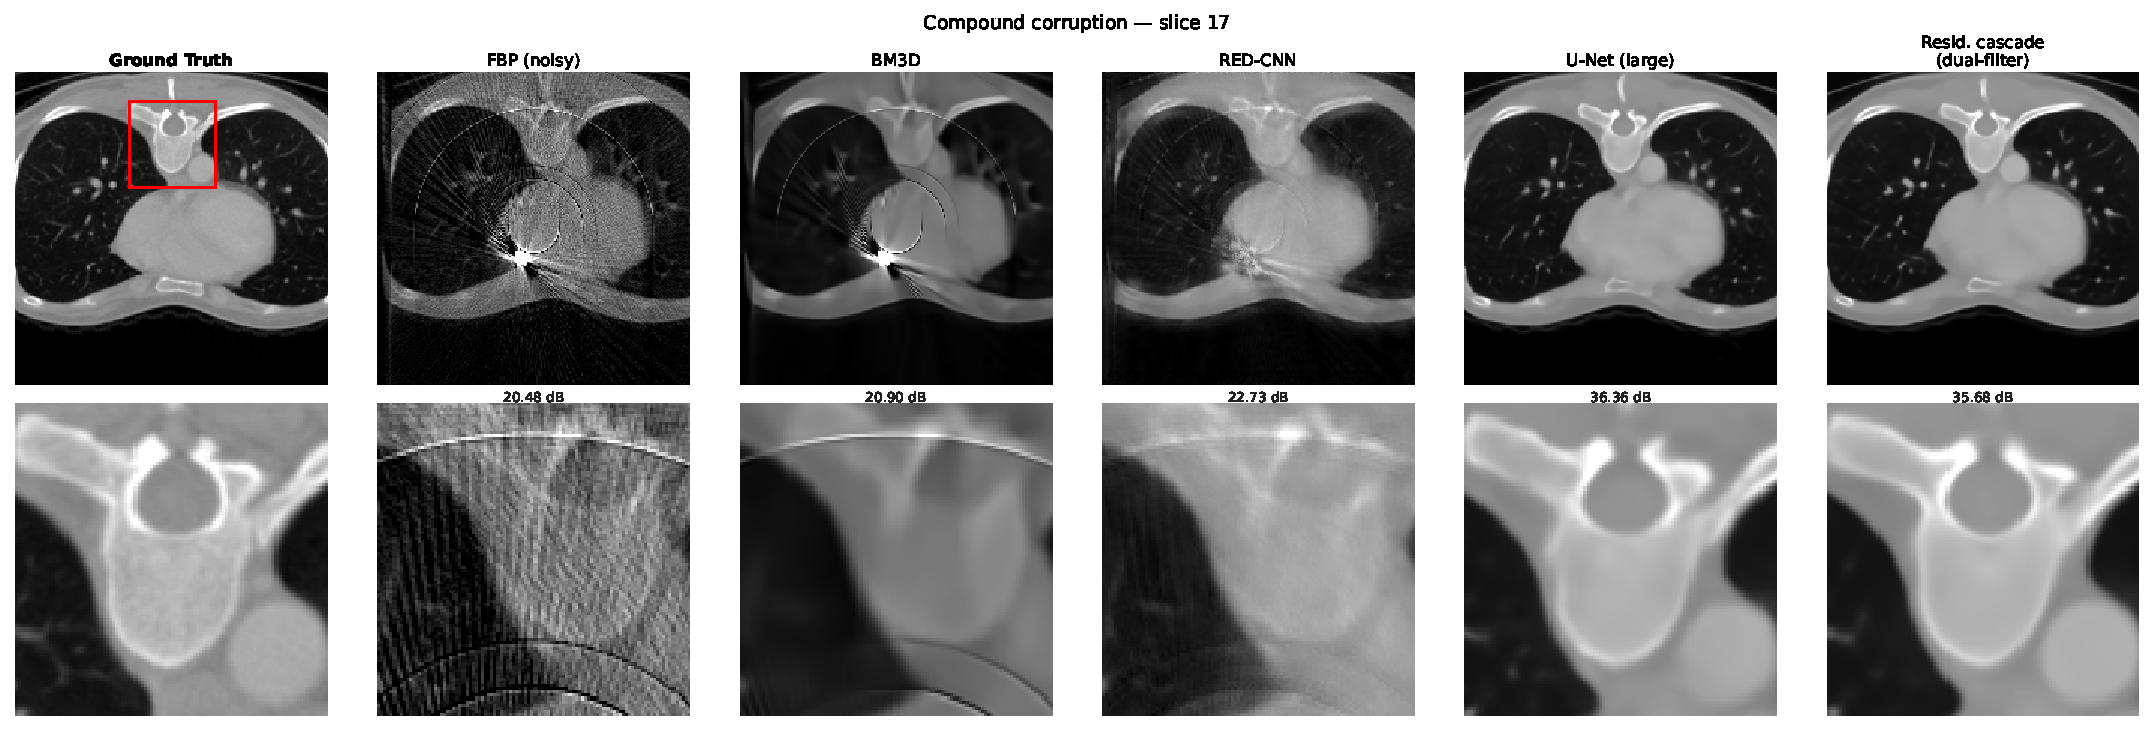
\includegraphics[width=\linewidth]{figures/results/fig_comparison_slice0017.pdf}
    \caption[Cross-method qualitative comparison under compound corruption (slice~17).]{%
        Qualitative comparison on slice~17 under compound corruption (Poisson noise,
        motion, ring, and metal artifacts co-occurring).
        \emph{Top row:} full reconstructions.
        \emph{Bottom row:} magnified crop of the highest-artifact region (red box on
        Ground Truth panel).
        PSNR~(dB) and SSIM are annotated beneath each column.
        BM3D suppresses diffuse noise but leaves structured streaks largely intact.
        RED-CNN removes most of the noise but struggles with metal streak saturation.
        The single-stage U-Net~(large) handles all artifact types effectively.
        The residual cascade with dual-filter input achieves the best visual
        suppression, most clearly visible in the zoomed crop near the streak
        boundaries. Supplementary per-artifact comparisons on additional slices
        are provided in \Cref{app:visuals}.}
    \label{fig:exp_qual_comparison}
\end{figure}

\Cref{fig:exp_qual_cascade} examines the cascade depth effect directly by showing the Stage~1 and Stage~2 outputs of all four cascade variants alongside the ground truth, together with a per-pixel difference map (Stage~2\,$-$\,Stage~1) on a diverging color scale. The difference maps share a common symmetric range across all rows, making the magnitude of Stage~2 corrections directly comparable.

\begin{figure}[!htb]
    \centering
    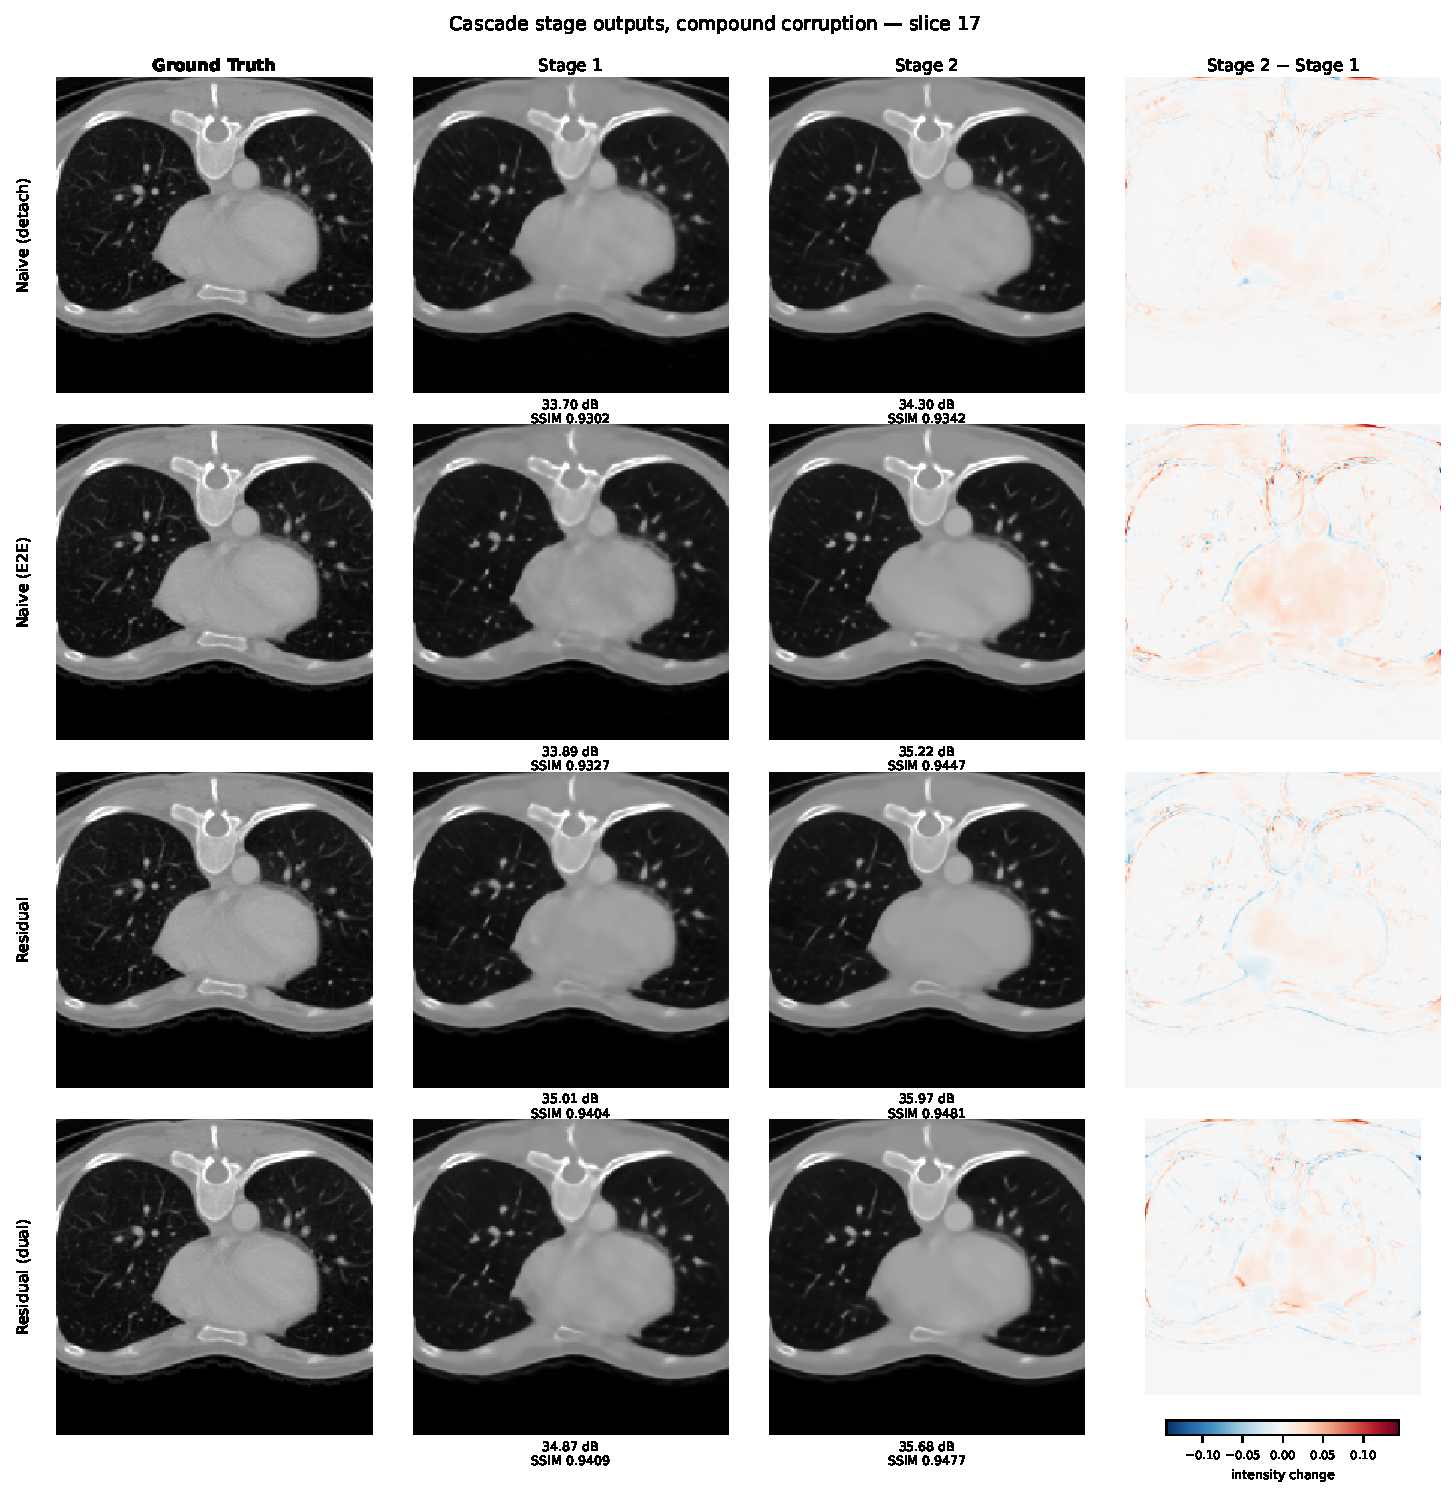
\includegraphics[width=\linewidth]{figures/results/fig_cascade_internals_slice0017.pdf}
    \caption[Cascade stage internals under compound corruption (slice~17).]{%
        Stage-by-stage outputs for all four cascade variants on slice~17 under
        compound corruption.
        \emph{Columns:} ground truth; Stage~1 output (PSNR/SSIM below);
        Stage~2 output (PSNR/SSIM below); per-pixel difference
        Stage~2\,$-$\,Stage~1 on a diverging color scale (blue~=~Stage~2 decreased
        intensity, red~=~increased; shared symmetric scale across all rows).
        In the naive cascade variants the difference maps show diffuse, spatially
        unstructured corrections of low magnitude, consistent with a Stage~2 that
        has received a weak gradient signal and has not learned a specialized
        corrective role.
        In the residual variants the corrections are more concentrated near
        artifact boundaries, with the dual-filter variant showing the most
        structured Stage~2 contribution.}
    \label{fig:exp_qual_cascade}
\end{figure}

The visual results corroborate the quantitative findings in \Cref{tab:exp_cascade}. BM3D reduces diffuse noise but leaves structured artifact signatures largely intact. The learned single-stage U-Net suppresses both noise and physical artifacts effectively, and the gap between the U-Net~(large) and the best cascade is small — visible primarily near metal streak saturation edges in the zoomed crop. The cascade internals figure reveals that the Stage~2 correction is modest across all variants, with the residual dual-filter model showing the most structured improvement, consistent with the $+0.72$\,dB gain reported in \Cref{tab:exp_cascade}.
%%─────────────────────────────────────────────────────────
%% Per-Stage Loss and Gradient Behavior
%%─────────────────────────────────────────────────────────
\section{Per-Stage Loss and Gradient Behavior}
\label{sec:exp_gradient}

To explain why deeper image-domain cascades do not surpass the effective single-network ceiling observed in \Cref{sec:exp_cascade}, the learning dynamics are examined at the level of individual stages.
\Cref{fig:exp_loss_curves} shows representative train and validation loss curves for four model variants, and \Cref{fig:exp_stage_improvement} summarizes the per-stage PSNR progression for the two strongest cascades.

\begin{figure}[!htb]
    \centering
    \begin{minipage}{0.48\linewidth}
        \centering
        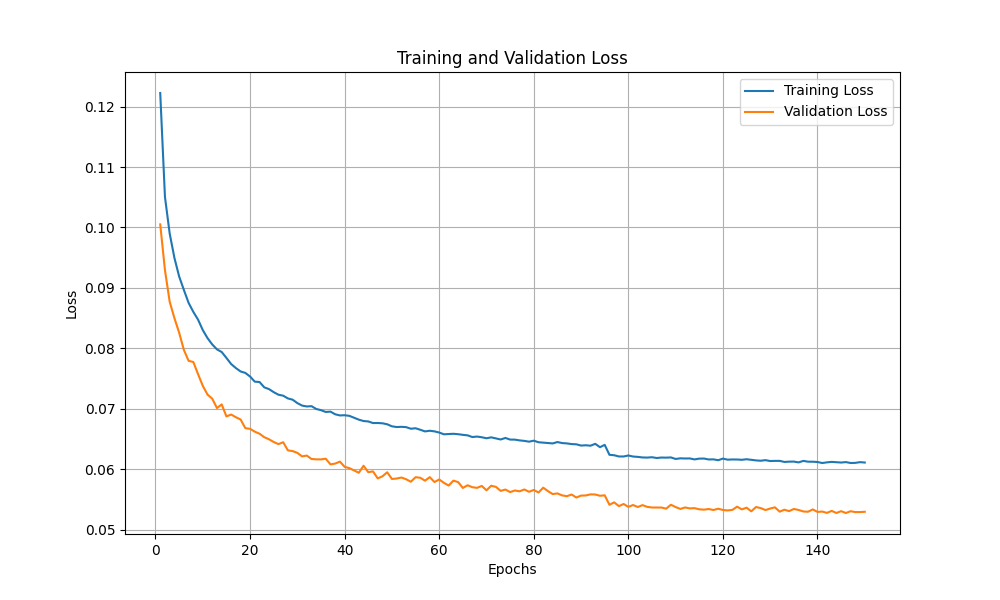
\includegraphics[width=\linewidth]{figures/results/loss_curves_unet_baseline.png}\\
        \footnotesize Single-stage U-Net.
    \end{minipage}\hfill
    \begin{minipage}{0.48\linewidth}
        \centering
        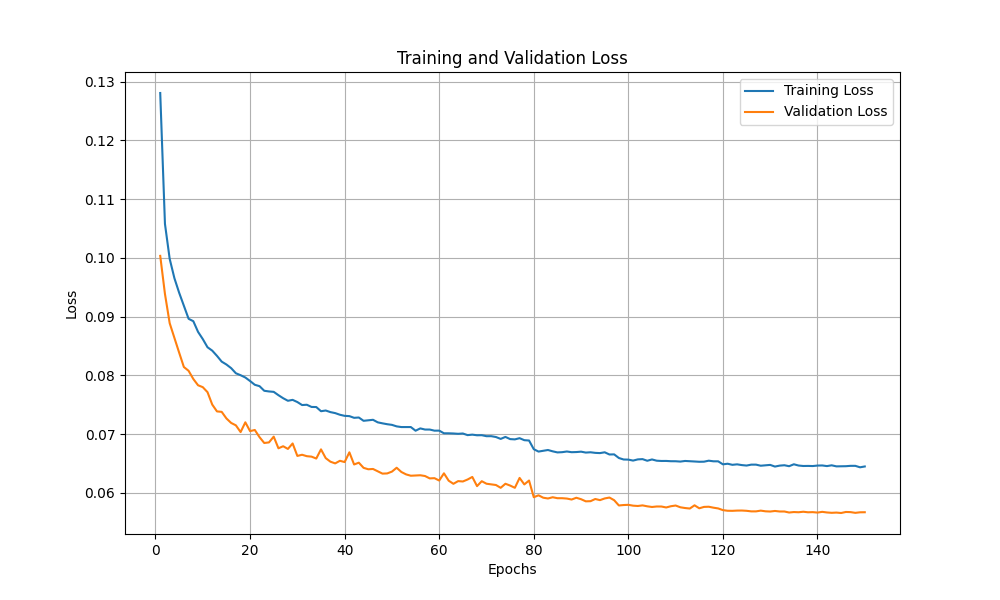
\includegraphics[width=\linewidth]{figures/results/loss_curves_naive_detach.png}\\
        \footnotesize Naive cascade, independent training.
    \end{minipage}\\[1.5ex]
    \begin{minipage}{0.48\linewidth}
        \centering
        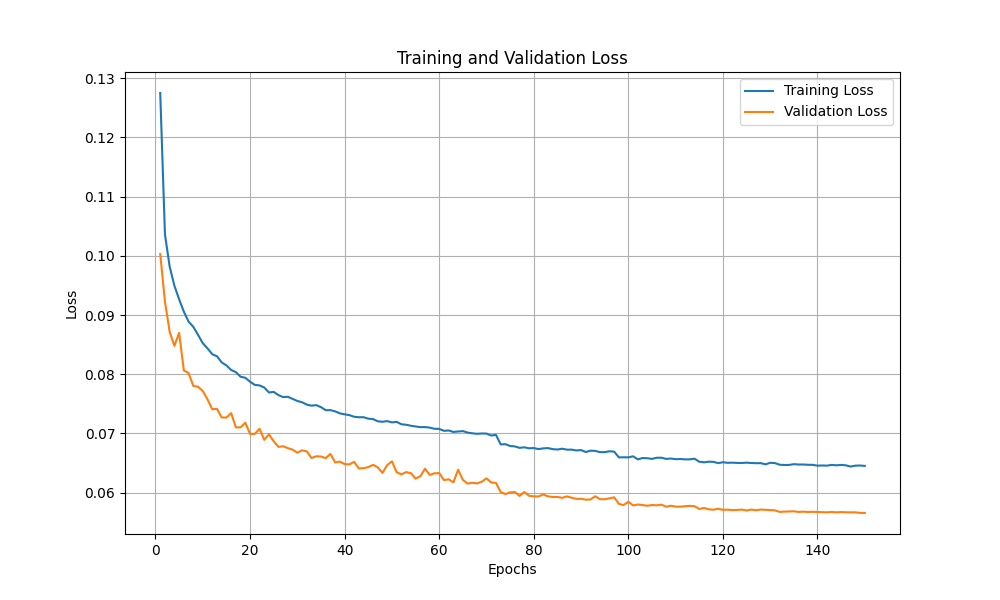
\includegraphics[width=\linewidth]{figures/results/loss_curves_naive_e2e.png}\\
        \footnotesize Naive cascade, end-to-end training.
    \end{minipage}\hfill
    \begin{minipage}{0.48\linewidth}
        \centering
        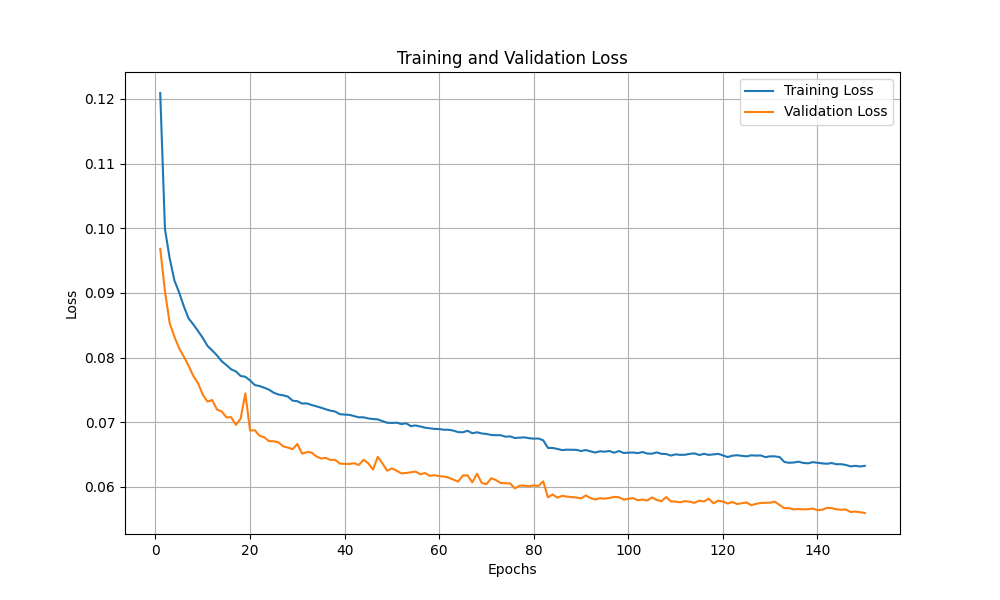
\includegraphics[width=\linewidth]{figures/results/loss_curves_residual_detach.png}\\
        \footnotesize Residual cascade, independent training.
    \end{minipage}
    \caption[Train/validation loss curves for representative variants.]{%
        Per-stage train and validation loss curves for four representative
        models. In all cascade variants, the Stage~1 loss plateaus near the
        same level reached by the single-stage U-Net, indicating that the
        first stage converges to a similar image-domain operating point.
        The Stage~2 loss of the residual cascade settles at a lower value,
        consistent with the smaller-magnitude residual target.}
    \label{fig:exp_loss_curves}
\end{figure}

The loss curves suggest that increased depth alone does not materially alter
the operating point reached by the first stage. Across the cascade variants,
Stage~1 converges to nearly the same loss level as the single-stage U-Net
trained in isolation. This indicates that the first stage already captures
most of the recoverable image-domain improvement under the present protocol,
leaving only a limited residual error for Stage~2 to model.

The residual cascade behaves differently only in the target presented to the
second stage. Because Stage~2 predicts a correction rather than a full clean
image, its optimization target has lower magnitude and is sparser in space.
The lower Stage~2 loss plateau is consistent with this reformulation and
provides one explanation for the stronger performance of the residual
variant in \Cref{tab:exp_cascade}.

\paragraph{Gradient attenuation in the end-to-end cascade.}
The end-to-end variant exhibits a marked attenuation of the Stage~2 learning
signal over training. The trainer logs the mean gradient magnitude for each
stage on the first batch of every epoch. In the small naive end-to-end
cascade, the Stage~2 gradient mean decreases from approximately
$\sim\!10^{-3}$ at initialization to $\sim\!10^{-4}$ within the first five
epochs and continues to decline thereafter, whereas the Stage~1 gradient
remains near the $3\times10^{-4}$ level.

By mid-training, the Stage~1/Stage~2 gradient-magnitude ratio reaches
approximately $3$--$5$. This indicates that the later stage receives a
progressively weaker optimisation signal as Stage~1 approaches its own
converged solution. In this setting, the second stage is not encouraged to
develop a strongly specialized corrective role, which helps explain why the
end-to-end naive cascade does not surpass the independently trained residual
variant in \Cref{tab:exp_cascade}.

\begin{figure}[!htb]
    \centering
    \begin{minipage}{0.48\linewidth}
        \centering
        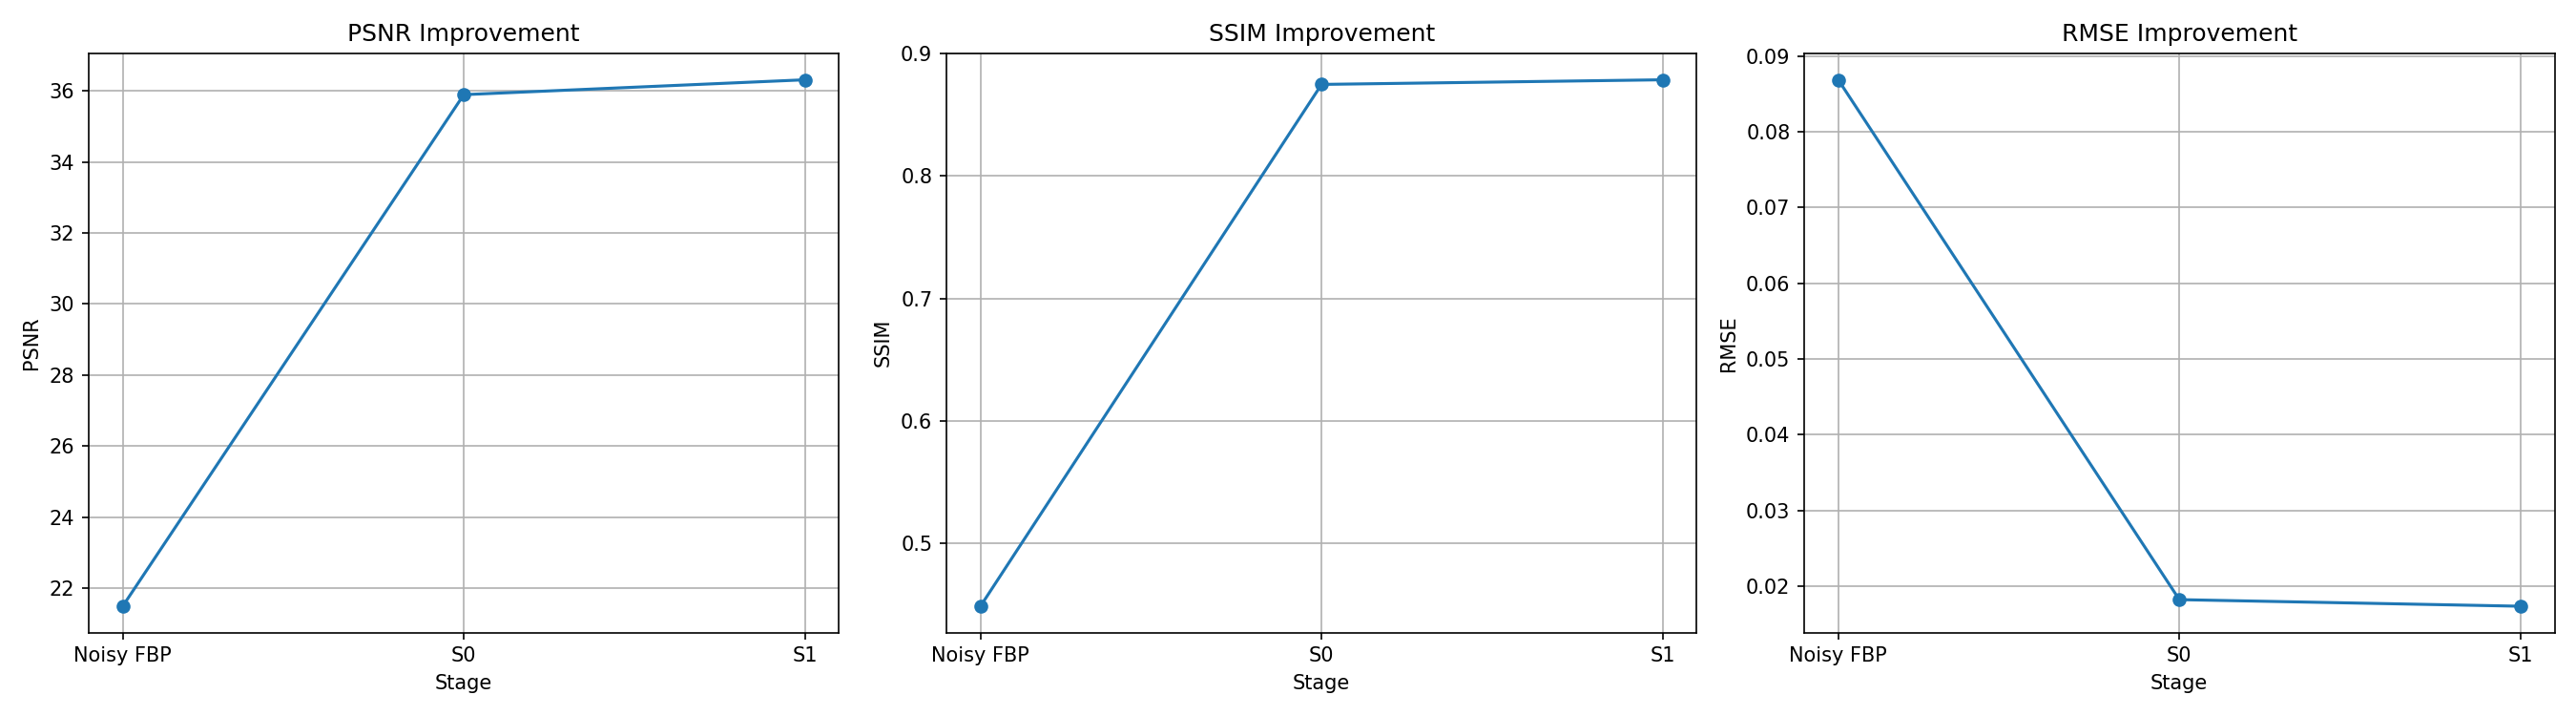
\includegraphics[width=\linewidth]{figures/results/stage_improvement_naive_large.png}\\
        \footnotesize Naive independent cascade (large+large).
    \end{minipage}\hfill
    \begin{minipage}{0.48\linewidth}
        \centering
        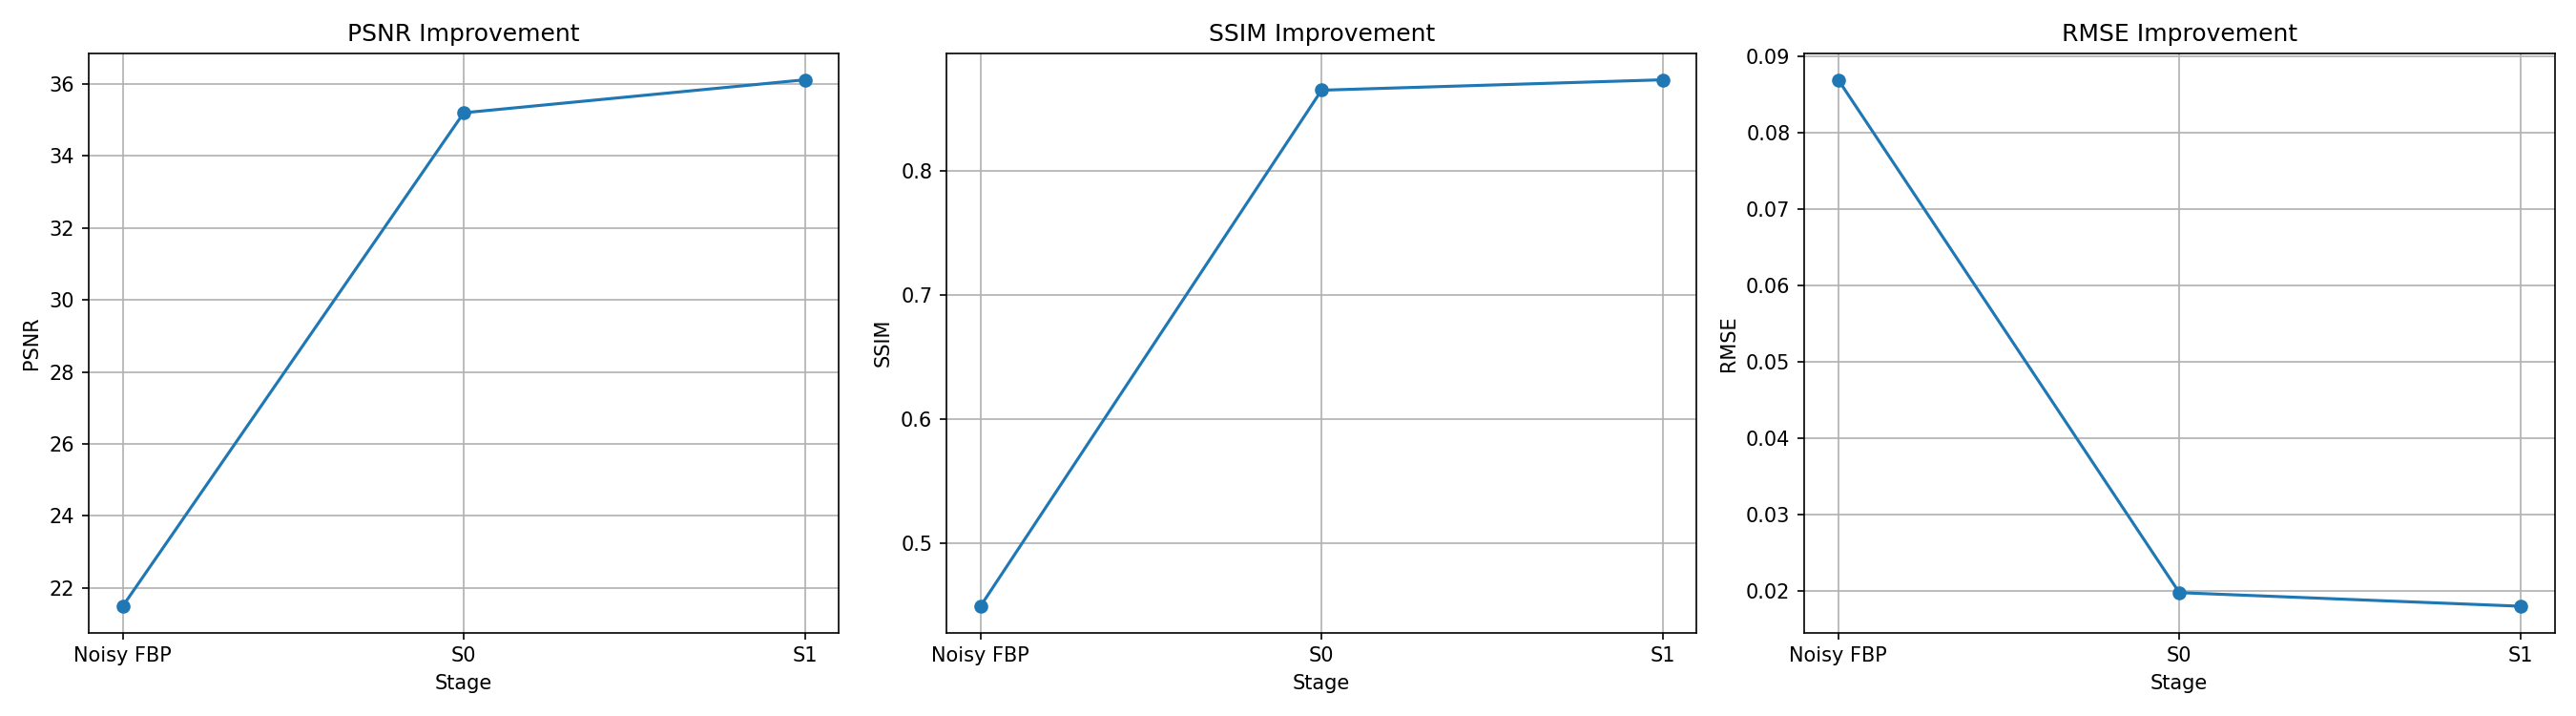
\includegraphics[width=\linewidth]{figures/results/stage_improvement_residual_dual.png}\\
        \footnotesize Residual independent cascade with dual-filter input.
    \end{minipage}
    \caption[Per-stage PSNR progression across the cascade.]{%
        PSNR at the corrupted FBP input, after Stage~1, and after Stage~2
        for the two strongest cascade variants. Most of the total
        improvement is achieved by Stage~1, while the Stage~2 increment is
        comparatively small and approaches the empirical image-domain ceiling
        discussed in \Cref{sec:exp_discussion}.}
    \label{fig:exp_stage_improvement}
\end{figure}

\FloatBarrier
%%─────────────────────────────────────────────────────────
%% Per-Stage Loss and Gradient Behavior
%%─────────────────────────────────────────────────────────
\section{Discussion}
\label{sec:exp_discussion}

\paragraph{An effective image-domain ceiling.}
The results suggest that a single well-designed encoder--decoder operating purely in the image domain already recovers most of the information that is practically recoverable from the FBP reconstruction under the present compound-corruption protocol. The empirical gap between the large single-stage U-Net (\SI{36.11}{\decibel}, SSIM~\num{0.8772}) and the best two-stage cascade in this study (\SI{36.11}{\decibel}, SSIM~\num{0.8738}, residual with dual-filter input) is zero in PSNR and only \num{0.0034} in SSIM. At matched per-stage capacity, the gain of the naive small$+$small cascade over the small single-stage U-Net is only \SI{0.15}{\decibel}. Taken together, these results indicate that simply increasing image-domain depth does not materially extend the attainable reconstruction quality on this protocol.

\paragraph{Why naive additional depth gives little benefit.}
The Stage~1 loss curves in \Cref{fig:exp_loss_curves} plateau at nearly identical values regardless of whether a second stage is attached. This suggests that Stage~1 already converges to essentially the same operating point as the corresponding single-stage model. The residual error that remains after Stage~1 therefore appears to be dominated by information that is not reliably recoverable from the corrupted image-domain input alone, including fine anatomical detail obscured by the combined effects of low photon flux and structured artifacts. Adding a second image-domain network does not change the information content of that input. In the end-to-end variant, this limitation is compounded by the gradient attenuation described in \Cref{sec:exp_gradient}, where the Stage~2 learning signal weakens as Stage~1 approaches convergence.

\paragraph{Residual configuration: empirical improvement and confounded factors.}
The residual cascade produces a consistent empirical improvement over the matched naive independent cascade ($+0.54$\,dB at symmetric small capacity). However, as noted in \Cref{subsec:meth_cascade_variants}, this configuration differs from the naive baseline along three axes simultaneously: the Stage~2 output representation (additive correction rather than direct image prediction), the Stage~2 loss function (residual $\ell^{1}$ plus SSIM plus gradient terms rather than balanced SSIM\,+\,$\ell^{1}$), and the Stage~2 backbone (ResUNet with intra-block shortcuts rather than plain U-Net). Without ablations that isolate each factor, the observed gain cannot be attributed to any single one of these changes.

Residual-learning arguments from image restoration suggest that predicting a lower-magnitude, sparser correction target should be easier to optimize than predicting the full clean image~\cite{Zhang2017}, and the additional gradient loss term is motivated by the metal-streak boundaries that pure SSIM\,/\,$\ell^{1}$ supervision tends to smooth over. Both are plausible contributors, but their individual contributions remain unresolved. The gain from the dual-filter input ($+0.18$\,dB over the standard residual cascade) is more cleanly interpretable, as it is the only difference between those two configurations: Stage~2 receives additional measurement-derived information that was not available in the single-channel case. Together, these modifications allow the cascade to approach the image-domain ceiling more closely, without removing it.

\paragraph{Information versus capacity.}
The asymmetric-capacity probe in \Cref{tab:exp_asym} indicates that final performance is influenced more by the quality of the intermediate representation than by the raw capacity of Stage~2 alone. Moving capacity from Stage~1 to Stage~2 reduces final performance, whereas strengthening Stage~1 and weakening Stage~2 changes the result only modestly. This provides the clearest evidence in the chapter that the second stage is constrained primarily by the residual information available to it rather than by insufficient downstream parameter count.

\paragraph{Per-artifact-count breakdown.}
\Cref{tab:exp_per_artifact} reports mean PSNR stratified by the number of co-occurring physical artifacts ($k = 0,1,2,3$) for all methods evaluated in this chapter. Artifact counts are determined by replaying the per-sample Bernoulli draws with the fixed test seed, yielding $n_{0}=584$, $n_{1}=1525$, $n_{2}=1185$, and $n_{3}=259$ slices in each stratum. All learned methods show a monotonic decrease in PSNR as artifact count increases. At $k=0$ (noise-only), PSNR values are highest for all methods and the spread between cascade variants is most pronounced. Performance differences across cascade formulations remain broadly consistent across strata, following the same ordering observed in the aggregate results of \Cref{tab:exp_cascade}.

\begin{table}[!htb]
    \centering
    \caption[Per-artifact-count PSNR breakdown for all evaluated methods.]{%
        Mean PSNR (dB) on the LoDoPaB-CT test split, stratified by the number of
        physical artifacts co-occurring in each test sample ($k=0$: noise-only;
        $k=1,2,3$: one, two, or three additional physical artifacts beyond the
        inherited Poisson noise). BM3D is not included per stratum as per-slice
        re-evaluation was computationally prohibitive; its aggregate PSNR is
        \SI{22.14}{\decibel}.}
    \label{tab:exp_per_artifact}
    \setlength{\tabcolsep}{5pt}
    \small
    \begin{tabular}{@{}l r r r r r@{}}
        \toprule
        Method & Overall & $k{=}0$ ($n{=}584$) & $k{=}1$ ($n{=}1525$) & $k{=}2$ ($n{=}1185$) & $k{=}3$ ($n{=}259$) \\
        \midrule
        Corrupted FBP               & $21.49$ & $24.08$ & $21.83$ & $20.28$ & $19.14$ \\
        RED-CNN~\cite{Chen2017}     & $27.03$ & $31.67$ & $27.61$ & $24.78$ & $23.19$ \\
        \midrule
        U-Net (small)               & $35.39$ & $39.37$ & $35.85$ & $33.56$ & $31.93$ \\
        \quad Naive indep.          & $35.54$ & $39.01$ & $35.97$ & $33.93$ & $32.48$ \\
        \quad Naive e2e             & $35.85$ & $39.45$ & $36.29$ & $34.16$ & $32.70$ \\
        \quad Residual              & $35.93$ & $39.56$ & $36.32$ & $34.27$ & $32.84$ \\
        \quad Residual + dual-filter& $36.11$ & $\mathbf{39.91}$ & $\mathbf{36.62}$ & $34.32$ & $32.63$ \\
        \midrule
        U-Net (large)               & $36.11$ & $39.64$ & $36.55$ & $\mathbf{34.47}$ & $\mathbf{32.99}$ \\
        \bottomrule
    \end{tabular}
\end{table}

\paragraph{Scope of the claim.}
These conclusions are based on depth-two cascades evaluated on LoDoPaB-CT under the specific compound-corruption protocol of \Cref{sec:meth_overview}. They should not be generalized automatically to architectures with explicit sinogram-domain processing, to datasets with substantially different anatomy or dose conditions, or to corruption regimes in which the post-Stage~1 residual retains richer exploitable structure. Even so, the dual-filter result points to the most promising direction observed in this study: the second stage becomes more useful when it receives information that is not already compressed into the Stage~1 output. A natural extension is therefore to combine image-domain refinement with an additional upstream branch that operates before reconstruction, as discussed in \Cref{chap:conclusion}.